
%%%
% Any line that begins with a percent symbol is a comment. To compile
% this document and view the output:
%
% Run Latex
% Run Bibtex
% Then run Latex twice.
%
% This should produce the output PDF file named main.pdf
%%%

% This defines the style to use for this document.
% Do not modify.
\documentclass[letterpaper]{article}

% The following are akin to "import" statements in Python or Java -
% these import useful commands into the document for you to use.  You
% don't have to modify any of these lines. The AAAI package formats
% this document in the style of submissions to the American
% Association for Artificial Intelligence conference, one of the top
% AI conferences in the world. You will find that many academic
% publications in AI use this format.
\usepackage{aaai} 
\usepackage{times} 
\usepackage{helvet} 
\usepackage{courier} 
\setlength{\pdfpagewidth}{8.5in} 
\setlength{\pdfpageheight}{11in} 
\usepackage{amsmath}
\usepackage{amsthm}
\usepackage{graphicx}
\usepackage{graphics}
\usepackage{moreverb}
\usepackage{subfigure}
\usepackage{epsfig}
\usepackage{txfonts}
\usepackage{palatino}
\usepackage{algpseudocode}
\usepackage{multirow, multicol}
\usepackage{url}
\usepackage{tablefootnote}
\usepackage{color}

\setcounter{secnumdepth}{1}
\nocopyright

% Fill in your paper title, names and emails below
% The "\\" is used to break lines. The \url command
% is useful for typesetting URLs and email addresses (it uses the
% Courier font).
\title{Solving the 15-Puzzle}
 \author{Alan Turing \and John von Neumann\\
 \url{{alturing, jovonneumann}@davidson.edu}\\
 Davidson College\\
 Davidson, NC 28035\\
 U.S.A.}

% This is the "true" start of the document. All the text in your
% write-up should be placed within the \begin{document} and
% \end{document} decorators.
\begin{document}

\maketitle % formats the title nicely, do not modify

% While at this point you could just begin your write-up, often, it's
% useful to write each section of your write-up in a separate tex
% file (not unlike the modular decomposition you do for code you
% write). These \input commands insert the contents of the
% specified tex files in the order specified. Every write-up you
% submit must contain the following sections, in the shown order. Open
% each of the indicated tex files to understand what goes in each
% section, as well as for more TeX tips.

% Place the contents of your abstract between the
% \begin{abstract} and \end{abstract} decorators.

\begin{abstract}

The abstract should be between four and seven sentences long. Introduce the
problem you are studying. Describe what you did. Summarize your results --- what
did you discover, what is the main take-away message?) Basically, you're trying 
to sell your paper to the reader, so be brief and to the point. \textbf{Do \emph{not}
include any citations in the abstract.}

% The \textbf{} command makes the specified text bold. The \emph{} or
% \textit{} command are used to italicize text. In general, text is never
% underlined.

% DON'T FORGET TO MATCH EACH OPEN BRACE WITH A CLOSING BRACE!
\end{abstract}



% The \section{} command formats and sets the title of this
% section. We'll deal with labels later.
\section{Introduction}
\label{sec:intro}

Linear, polynomial, and other forms of regression analysis are commonly
used in the field of statistics in order to fit a function to a data set. Produced
functions can be used to predict behavior at arbitrary input values. Typically,
regression analysis is used upon data sets for which the approximate
function \textit{type} (e.g. linear, quadratic, etc.) is known. Traditional
regression analysis is not well-suited, however, for data sets which
approximate an unknown function type. \\

One tried solution for such scenarios is symbolic regression by way of
a genetic algorithm --- an algorithm that generates sets of candidate
solutions, randomly splices together traits from pairs of fit "parents"
into "children" over successive generations, and occasionally mutates
pieces of those candidates, until a strongly fit solution is found. \\

In our paper we introduce expression trees as a means of representing
functional expressions in such a way that they can be easily spliced by
a genetic algorithm. We discuss our own implementation of symbolic
regression for two known data sets representing unknown functions,
inspired by the work of John Koza. \cite{examplerun}



\section{Background}
\label{sec:background}

Describe any background information that the reader would need to know
to understand your work. You do not have to explain algorithms or
ideas that we have seen in class. Rather, use this section to describe
techniques that you found elsewhere in the course of your research,
that you have decided to bring to bear on the problem at hand. Don't
go overboard here --- if what you're doing is quite detailed, it's
often more helpful to give a sketch of the big ideas of the approaches
that you will be using. You can then say something like ``the reader
is referred to X for a more in-depth description of...'', and include
a citation.\\

Alternately, you may have designed a novel approach for the problem
--- your own algorithm or heuristic, say. A description of these would
also be placed in this section (use subsections to better organize the
content in this case).

% Note the \subsection{} command 
\subsection{Enumerating}
\label{subsec:enum}

Create bulleted lists by using the \texttt{itemize} command (see source code):
\begin{itemize}
  \item Item 1
  \item Item 2
  \item Item 3
\end{itemize}
Create numbered lists by using the \texttt{enumerate} command (see source code):
\begin{enumerate}
  \item Item 1
  \item Item 2
    \begin{enumerate}
    \item Sub-item 2a
    \item Sub-item 2b
    \end{enumerate}
  \item Item 3
\end{enumerate}

\subsection{Formatting Mathematics}
\label{subsec:math}

Entire books have been written about typesetting mathematics in
\LaTeX~, so this guide will barely scratch the surface of what's
possible. But it contains enough information to get you started, with
pointers to resources where you can learn more. First, the basics: all
mathematical content needs to be written in ``math-mode'' --- this is
done by enclosing the content within \$ symbols. For example, the code
to produce $6x + 2 = 8$ is \texttt{\$6x + 2 = 8\$}. Note that this is
only good for inline math; if you would like some stand-alone math on
a separate line, use \emph{two} \$ symbols. For example,
\texttt{\$\$6x + 2 = 8\$\$} produces: $$6x+2 = 8$$ Here are various
other useful mathematical symbols and notations --- see the source
code to see how to produce them.

\begin{itemize}
  \item Sub- and super-scripts: $e^{x}, a_{n}, e^{2x+1}, a_{n+2}, f^{i}_{n+1}$
  \item Common functions: $\log{x}, \sin{x}$
  \item Greek symbols: $\epsilon, \phi, \pi, \Pi, \Phi$ % capitalizing the first letter produces the upper case letter
  \item Summations: $\sum_{i=0}^{i=100} i^{2}$ % looks nicer if you typeset it on its own line using $$
  \item Products: $\prod_{i=0}^{\infty} 2^{-i}$
  \item Fractions: $3/2$ % prefer this look for inline math
    $$\frac{x + 5}{2 \cdot \pi}$$\\ % only looks nice when typeset on its own line
\end{itemize}

\noindent Other useful resources:
\begin{itemize}
\item Find the \LaTeX~command you're looking for by drawing what you
  want to produce\footnote{Thanks to Dr. Kate Thompson for pointing me
    to this resource. Also, this is how you create a footnote. Also,
    don't overuse them --- prefer citations and use the
    acknowledgements section when possible. I usually only use
    footnotes when I want to link to include a pointer to a web
    site.}:\url{http://detexify.kirelabs.org/classify.html}
\item Ask others: \url{http://tex.stackexchange.com/}
\item Every \LaTeX~symbol ever:\\ \url{http://tinyurl.com/6s85po}

\end{itemize}




\section{Experiments}
\label{sec:expts}

In this section, you should describe your experimental setup. What
were the questions you were trying to answer? What was the
experimental setup (number of trials, parameter settings, etc.)? What
were you measuring? You should justify these choices when
necessary. The accepted wisdom is that there should be enough detail
in this section that I could reproduce your work \emph{exactly} if I
were so motivated.


\section{Results}
\label{sec:results}

In order to help the algorithm converge on the correct solutions, the parameters guiding the behavior of the algorithm were tailored to increase population diversity, maintain successful trees, and correctly adapt to the goal functions.  The sampling range of the functions also had significant impact on the algorithm's accuracy.  When comparing an expression tree to the goal functions, which determined the fitness of the trees, best results were seen when the error was calculated over a range where the goal function was significantly non-zero.  If the fitness was calculated over larger ranges of input values, the expression trees tended strongly towards constant expressions that minimize total error but describe only the asymptotic tails of the function.  

Data points taken from the first goal function are displayed in Figure~\ref{tab:fcn1}.  The second goal function is four dimensional, and cannot be conveniently displayed.

\begin{figure}
\centering
	\begin{tikzpicture}
		\begin{axis}
			\addplot[scatter, only marks] table [x=x, y=y, col sep=space] {data1_small.txt};
		\end{axis}
	\end{tikzpicture}
\caption{Non-zero section of goal function 1}
\label{tab:fcn1}
\end{figure}

Despite careful adjustment of parameters governing tree construction, mutation rate, and the sampling range of the fitness function, we were unable to develop any non-constant expressions for the goal functions as given.  While closing the sampling range to only include the area of the fitness function displaying interesting, non-asymptotic behavior did result in lower error amongst the most accurate trees, the genetic algorithm was unable to determine a more accurate function.  

As another approach to solving the first function, we took the reciprocal of the output of the goal function in order to alter the expression needed to produce it.  Surprisingly, this met with success, as the algorithm consistently finds $x^2$ solutions which closely approximate the goal function.  Unlike the runs with the original goal function, the fitness scores converge when evaluating based on the inverted function.  Through this technique, we were able to arrive at an accurate function, which we then invert to conclude that the first goal function is 
	$$ y = \frac{10}{x^2- 6x + 14} $$

Unfortunately, this technique has not been successful for the second goal function, which has 3 input variables.  For that reason, we were also unable to plot the data in order to determine an appropriate sampling region or to visualize the function in general.  When attempting to fit the second goal function, our algorithm always relies on a constant function.  Unfortunately, this is clearly not a correct solution, as the error associated with such trees is massive.

%Present the results of your experiments. Simply presenting the data is
%insufficient! You need to analyze your results. What did you discover?
%What is interesting about your results? Were the results what you
%expected? Use appropriate visualizations. Prefer graphs and charts to
%tables as they are easier to read (though tables are often more
%compact, and can be a better choice if you're squeezed for space).
%\textbf{Always} include information that conveys the uncertainty in
%your measurements: mean statistics should be plotted with error bars,
%or reported in tables with a $\pm$ range. The $95\%$-confidence
%interval is a commonly reported statistic.

%\subsection{Embedding Pictures}
%\label{subsec:pics}

%See the source code (\texttt{results.tex}) for instructions on how to
%insert figures (like figure~\ref{fig:tex}) or plots into your
%document.

% Note that TeX has a mind of its own when it comes to placing images
% in documents - where a figure appears in the PDF document will often
% be quite different from where it appears in the source code. This is
% a feature, not a bug - it enables LaTeX to produce layouts that
% "flow" better. It only takes a few lines to insert a figure into
% your write-up - I recommend using PNG, JPG or PDF images
% (incidentally, programs like Excel and Matlab will allow you to save
% any plots or figures you generate in those formats). The \figure{}
% command is used to create a new figure.
%\begin{figure}[htb]

%  \centering  % centers the image in the column

  % replace the second argument below with your filename. I like to
  % place all my figures in a sub-directory to keep things organized
%  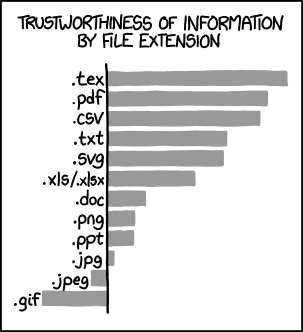
\includegraphics[width=0.47\textwidth]{figs/file_extensions.png}

  % *Every* figure should have a descriptive caption.
%  \caption{On the trustworthiness of \LaTeX. Image courtesy of \texttt{xkcd}.}

  % The label is a handle you create so that you can refer to this
  % figure (using the \ref{} command) from other parts of your
  % document. LaTeX automatically renumbers figures and updates
  % references when you recompile, so you should do it this way rather
  % than hard-coding in references. Notice that I've also been
  % creating labels for the various sections in the document; I could
  % use \ref{} command to refer to those sections using their labels
  % too.
%  \label{fig:tex}

%\end{figure}

%\subsection{Creating Tables}
%\label{subsec:tables}

%Again, refer to \texttt{results.tex} to learn how to create simple
%tables (like table~\ref{tab:example}).
%\begin{figure}[htb]
%  \centering % centers the entire table

  % The following line sets the parameters of the table: we'll have
  % three columns (one per 'c'), each
  % column will be centered (hence the 'c'; 'l' or 'r' will left or
  % right justify the column) and the columns
  % will have lines between them (that's the purpose of the |s between
  % the 'c's).
%  \begin{tabular}{|c|c|c|} 
%    \hline \hline % draws two horizontal lines at the top of the table
%    Column 1 & Column 2 & Column 3 \\ % separate column contents using the &
%    \hline % line after the column headers
%    $1$ & $3.1$ & $2.7$ \\
%    $42$ & $-1$ & $1729$\\
%    \hline \hline
%  \end{tabular}

  % As with figures, *every* table should have a descriptive caption
  % and a label for ease of reference.
%  \caption{An example table.}
%  \label{tab:example}

%\end{figure}



\section{Conclusions}
\label{sec:concl}

In this experiment, we used a genetic algorithm for symbolic regression against two unknown goal functions.  We developed a population of expression trees through 50 generations by evaluating the trees' fitness via their error against the goal function.  Though this approach did not autonomously solve the goal functions, data manipulation -- in the form of taking the reciprocal of the output of the goal function -- allowed the algorithm to correctly solve one of the functions.  While the variability and potential solving power of genetic programming can seem a catch-all solution, our results indicate that careful data analysis may be needed to supplement the algorithm in order for it to be effective.  This problem deserves further research by this team in order to determine a more robust solution to the single input problem and to solve the more complex three input problem.


\section{Acknowledgements} 
\label{sec:ack} 

This section is optional. But if there are people you'd like to thank for their help with the project --- a person who contributed some insight, friends who volunteered to help out with data collection, etc. --- then this is the place to thank them. Keep it short!


% This creates the references section. Open the project1.bib file to
% see how to organize your references.
\bibliography{project1}
\bibliographystyle{aaai} % sets citation and bib style, do not modify

\end{document}
